\documentclass{article}
\usepackage{amsmath,graphicx,amssymb,amsthm,url,listings}

\newcommand\tab[1][1cm]{\hspace*{#1}}

\title{Implementation Assignment 3}
\date{\today}
\author{Rong Yu and Finn Womack}

\begin{document}
	\maketitle
	\section*{Part I: K-NN}
	\subsection*{1.1: Normalizing data and implementing K-NN}
After loading the testing and training data into feature matrices and vectors we normalized the data by calculating the minimum value, and the range $(max - min)$ of the training data for each feature and then normalized both the testing and training data using the training values
	
	Then we created a function that implements the K-NN algorithm with training data $($ features and outputs $)$, testing features, and k as parameters.
	
	\subsection*{1.2: Running K-NN}
	We then iterated over the following values of k:
	
	$$
	\{ K \in \mathbb{Z} \cap [0,70] | K \ is \ odd \}
	$$
	
	For each value of K we then calculated the training and testing errors as well as the leave-one-out cross validation error. We then normalized the training and testing errors to a ratio so that the graph would be comparable when plotted on the following graph:
	
	\newpage
	
	\begin{figure}[h!]
		\begin{center} 
			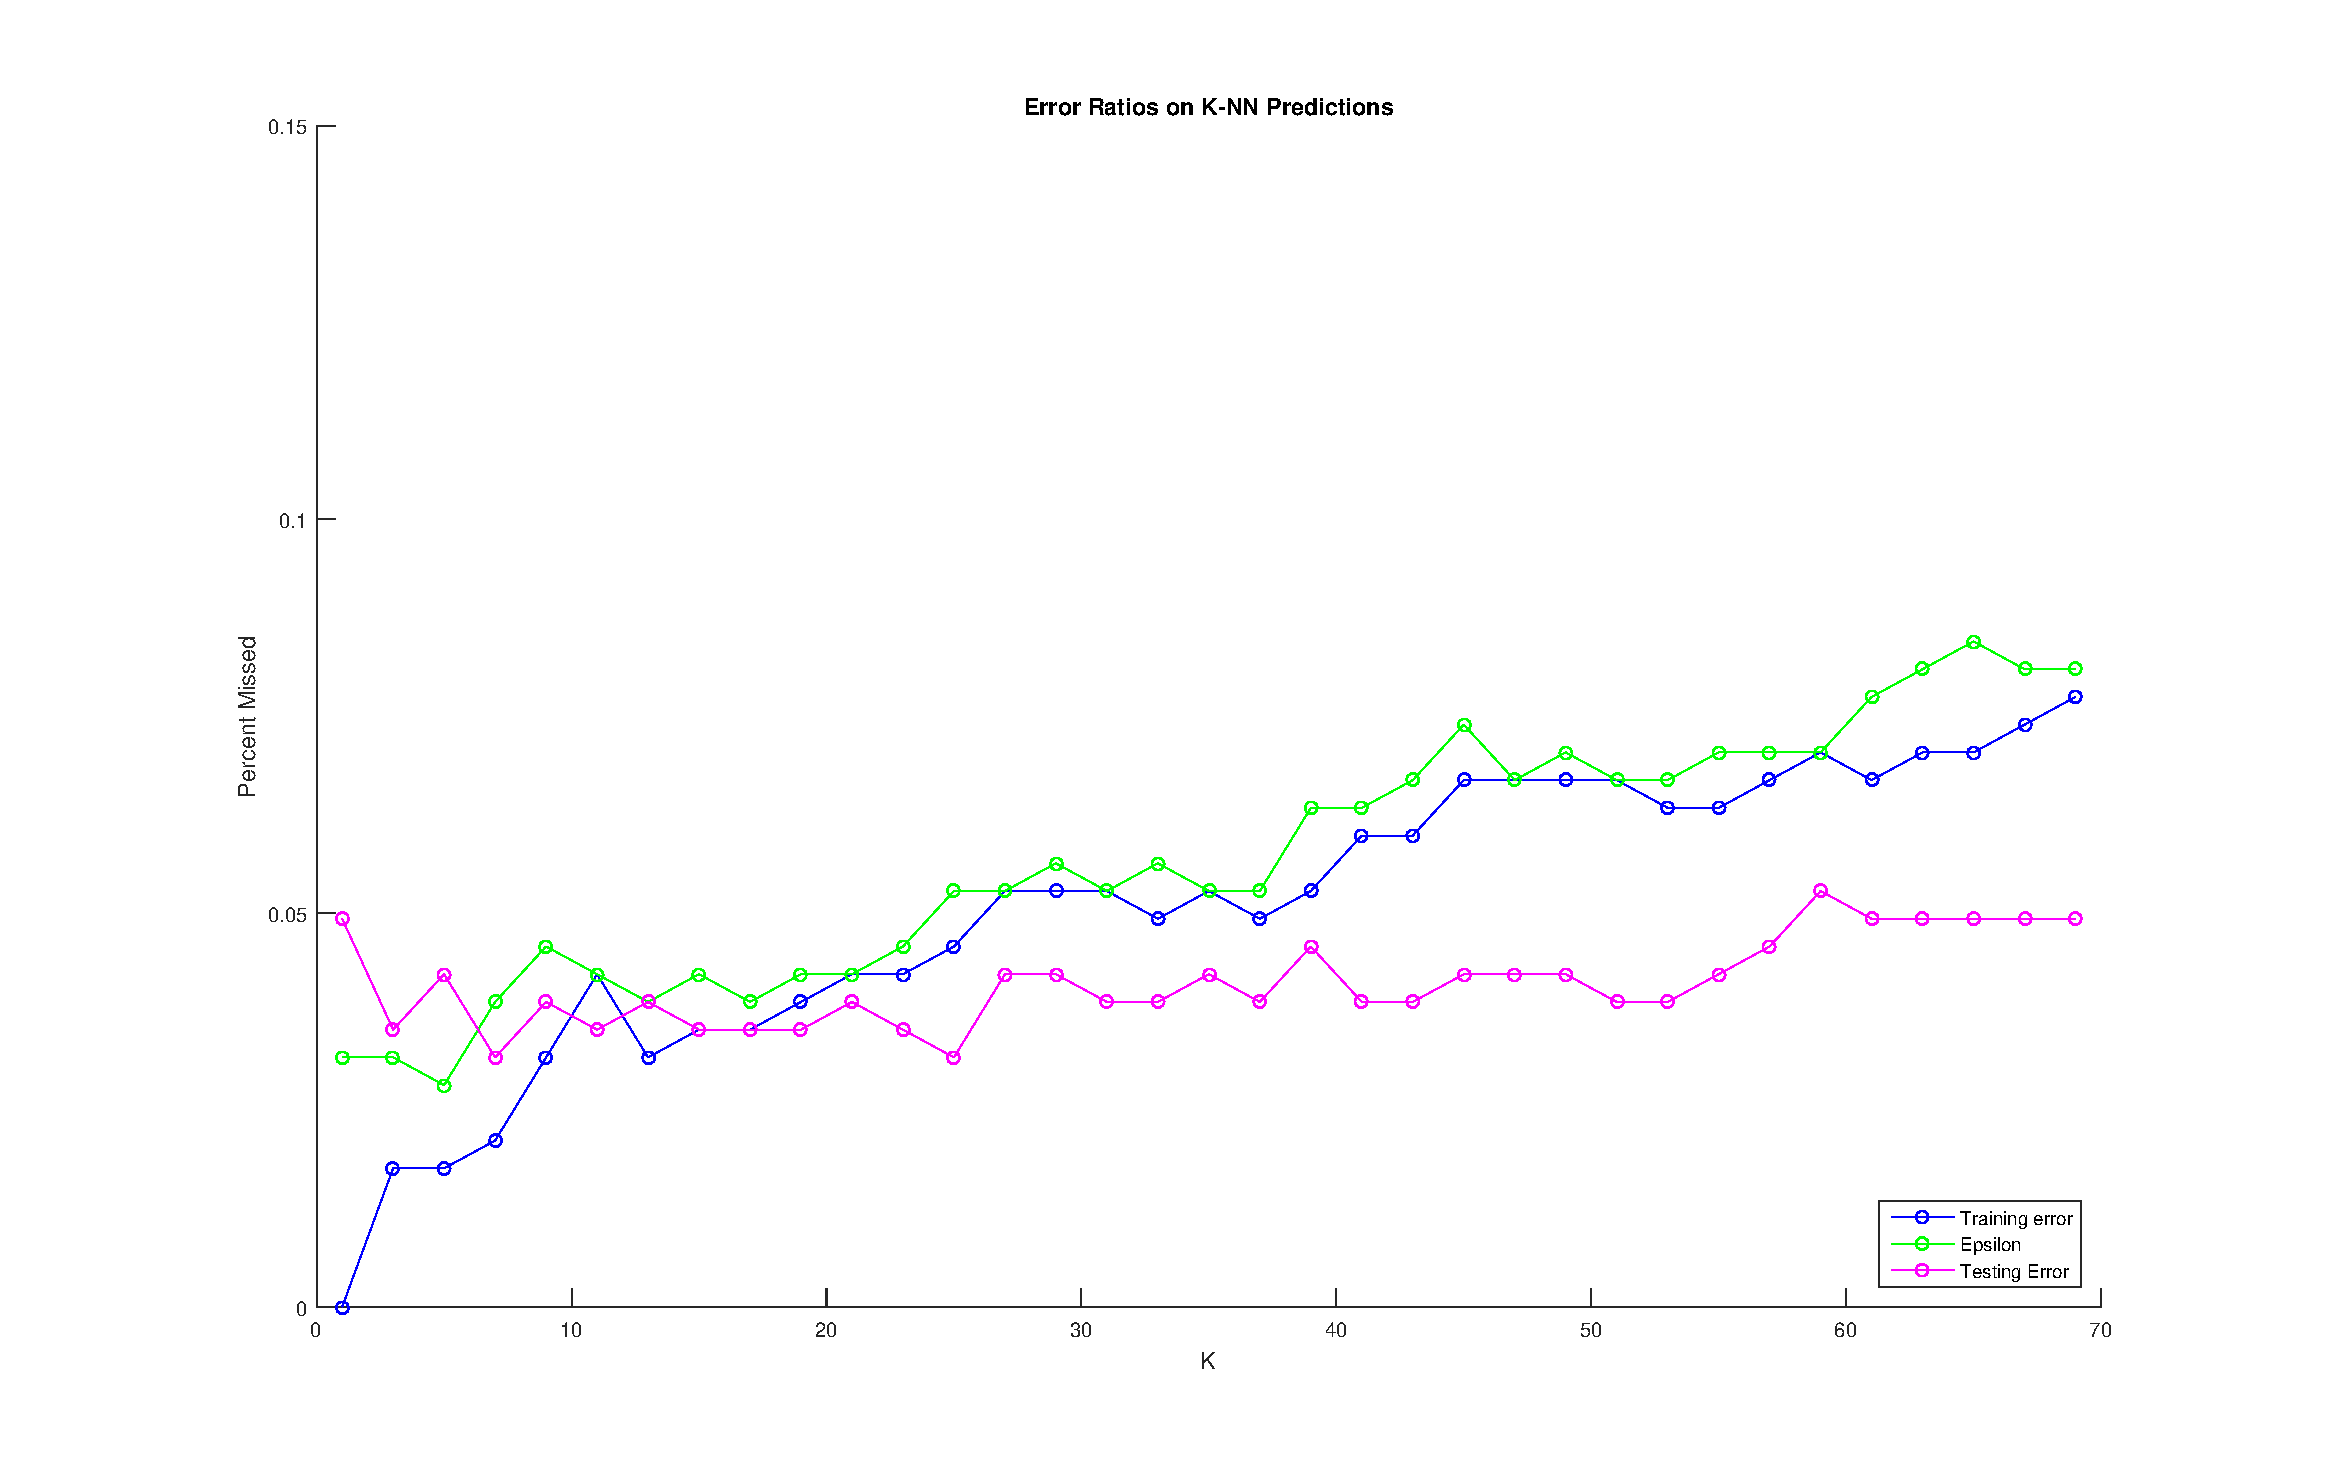
\includegraphics[scale=0.4]{knn.eps} 
		\end{center} 
		\label{fig:M1}
	\end{figure}
	
	From the above graph we can see that Training error is minimized at $K = 7 \ \& \ K = 25$. Also, we can see that training error steadily climbs as K grows. Lastly, we can see that the cross validation error is minimized at $K = 5$. 
	
	
	Cross validation error appears to be related both testing and training error but is more dominantly effected by training error. At first the training error increases while cross validation and testing error decreases. This makes sense because as we generalize the model it will over-fit less. However, past a certain point the increasing K starts to cause under-fitting in the model increasing errors across the board. 
	
	Looking at both the cross validation error and the testing error into account we would choose $K = 7 $ because it minimizes both quantities the best. Also, even if just looking at testing data we would choose $K = 7$ because, while $K = 25$ also minimizes the testing error, $K = 7$ reduces the complexity of the model resulting in a better overall model. If we didn't have testing data and we just looking at cross validation error we would of course choose $K = 5$ since it minimizes the cross validation error.
	
	\newpage
	
	\section*{Part II: Decision Tree}
	
	\subsection*{2.1: Decision Stump}
	
	After writing a function for the decision stump we calculated the number of errors in the training data and testing data and got the following results:
	
	\begin{align}
		Error_{testing} &= 26\\
		Error_{training} &= 22
	\end{align}
	
	The decision stump seems to preform pretty well despite only having a decision.
	
	\subsection*{2.2: Exploring Depth}
	
	We implemented the decision tree algorithm using the decision stump function. We then generated decision trees for the depths $1, 2, 3, ..., \& 10$. The diagram we made for the 6th layer tree is included in the turned in .zip file as a jpeg. We then calculated and plotted the training and testing error rates for each depth and this gave the following plot:
	
	
	\begin{figure}[h!]
		\begin{center} 
			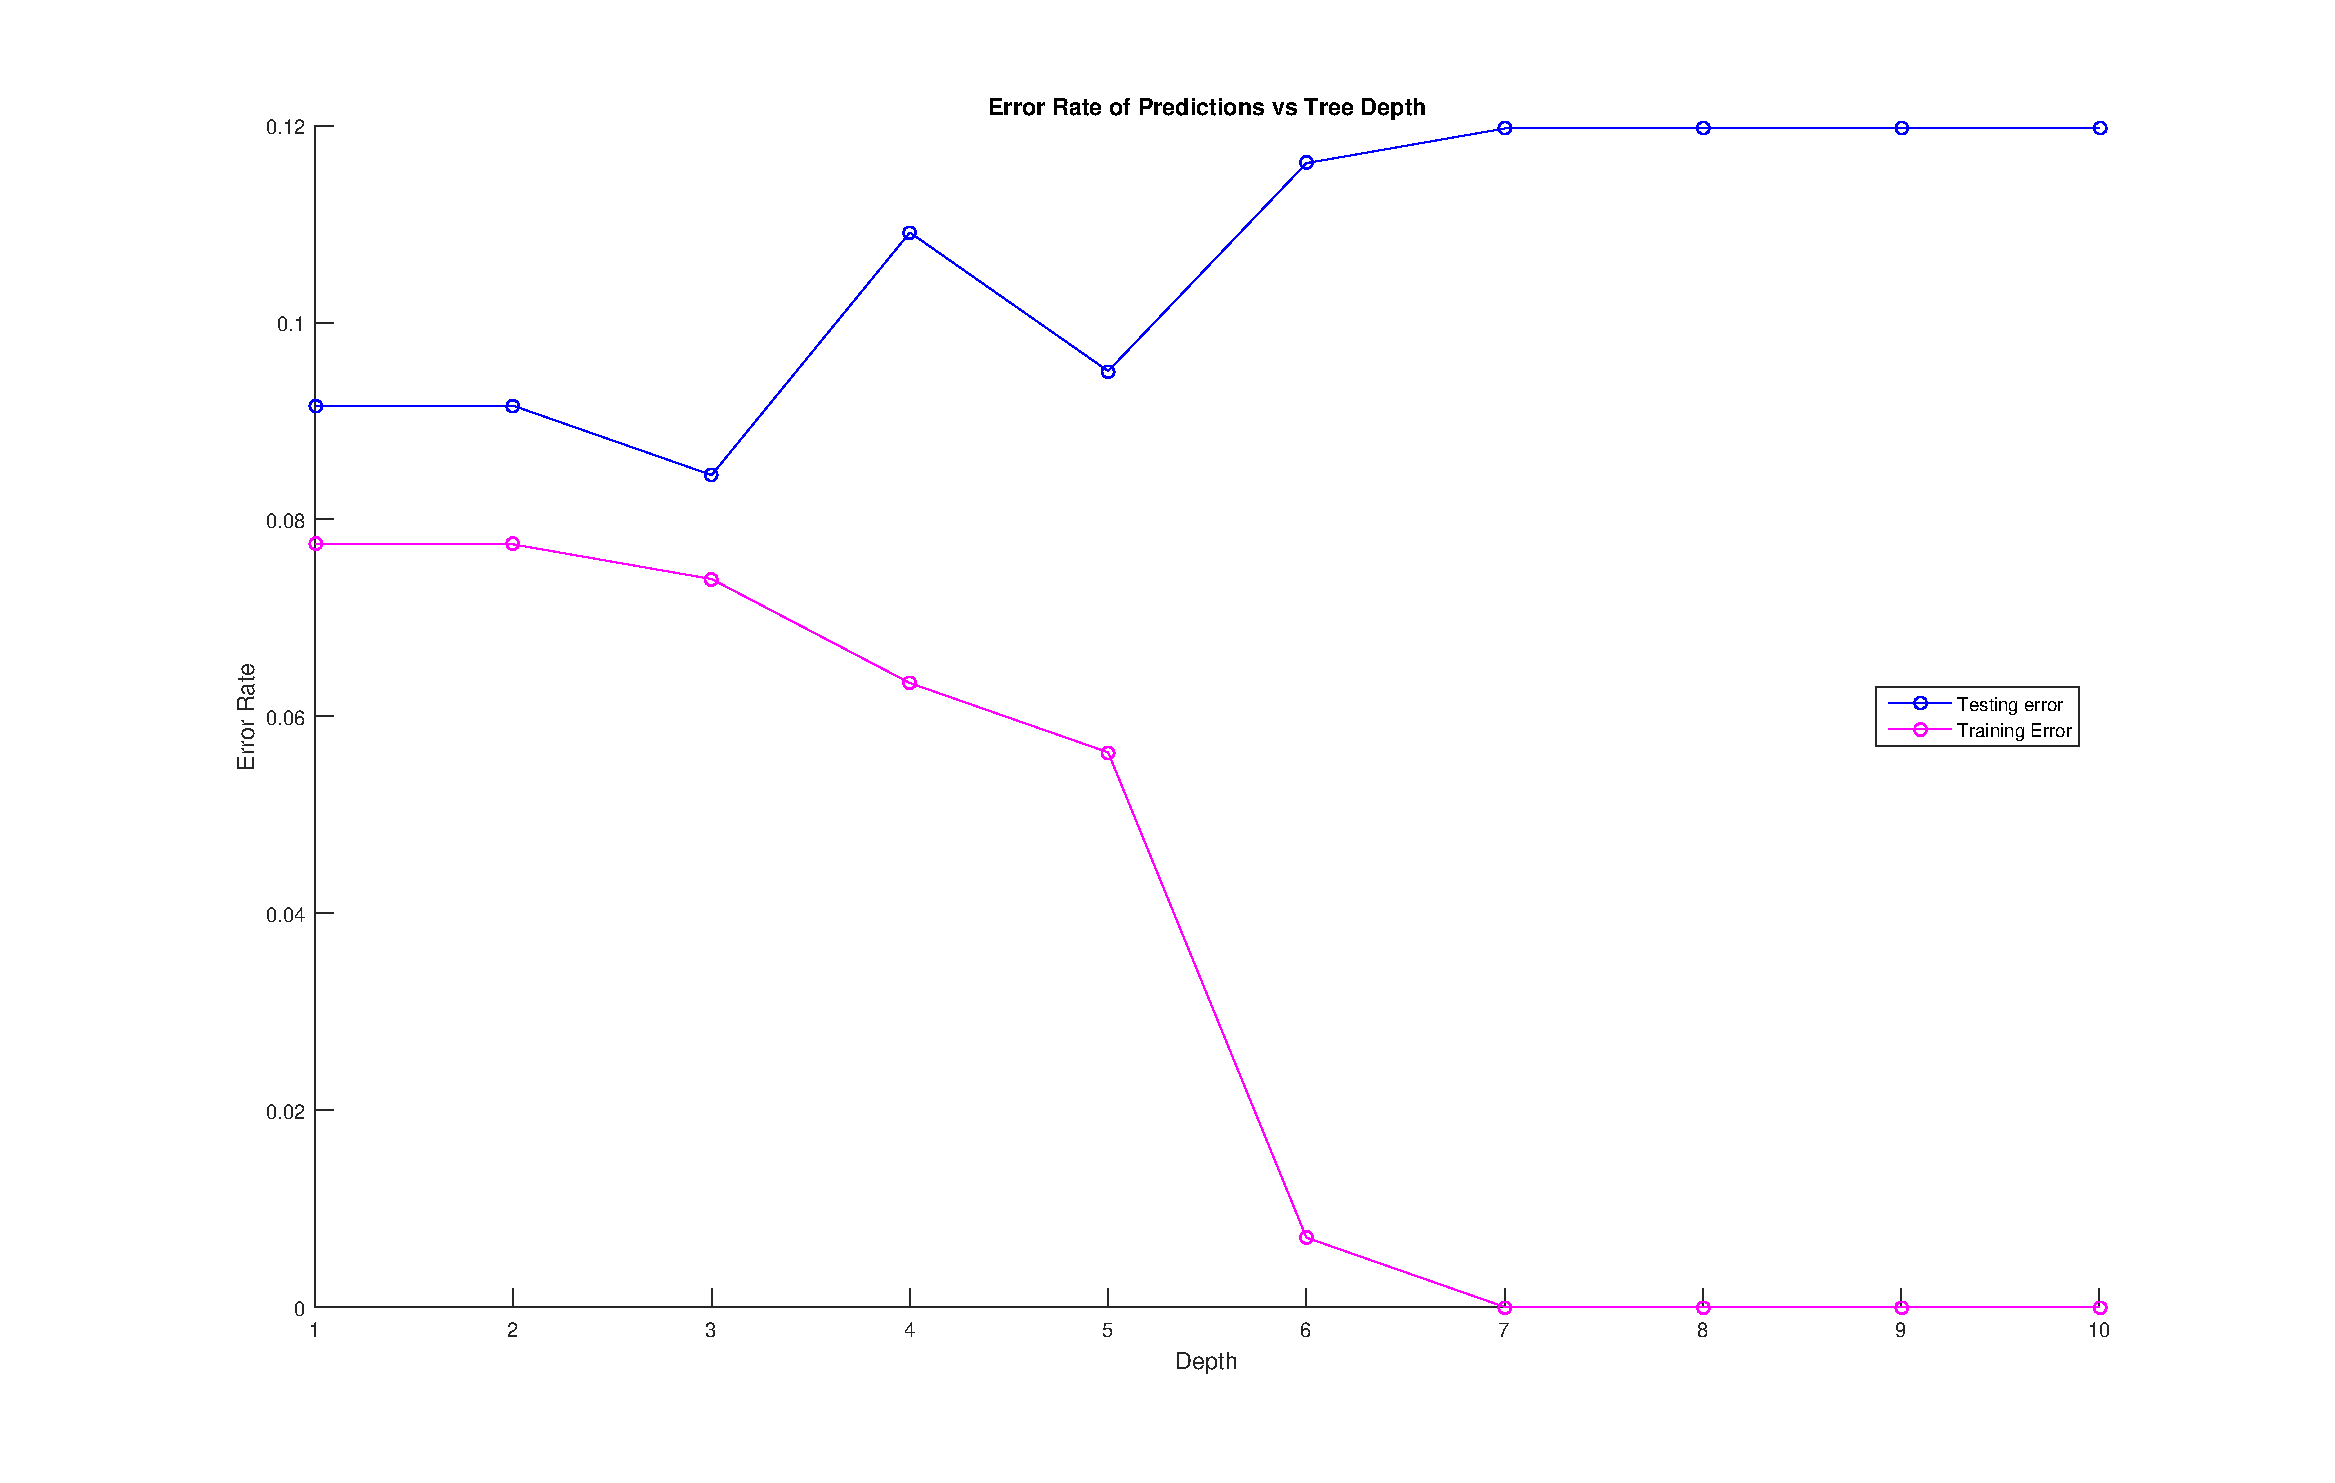
\includegraphics[scale=0.4]{depth.eps} 
		\end{center} 
		\label{fig:M2}
	\end{figure}
	
	\newpage
	
	As we can see the the stump does a relatively good job but as the depth increases the errors decrease until the testing error begins to increase again as the model begins to over-fit the training data. This makes sense as the more developed the tree is the better it will fit the training data until it fits it perfectly. It appears that a tree with a depth of 3 preforms the best on the testing data.
	
	\section*{Part III: Extra Credit}
	

	

	
	Since the K-NN algorithm is not very robust to junk features we thought that we might be able to improve the performance by looking at the features used in a 3rd layer decision tree and using that to trim the features used in K-NN. This tree used the features 12, 19, 23, 27, 28, and 30. We then repeated the process in part I and generated the following graph:
	
	\begin{figure}[h!]
		\begin{center} 
			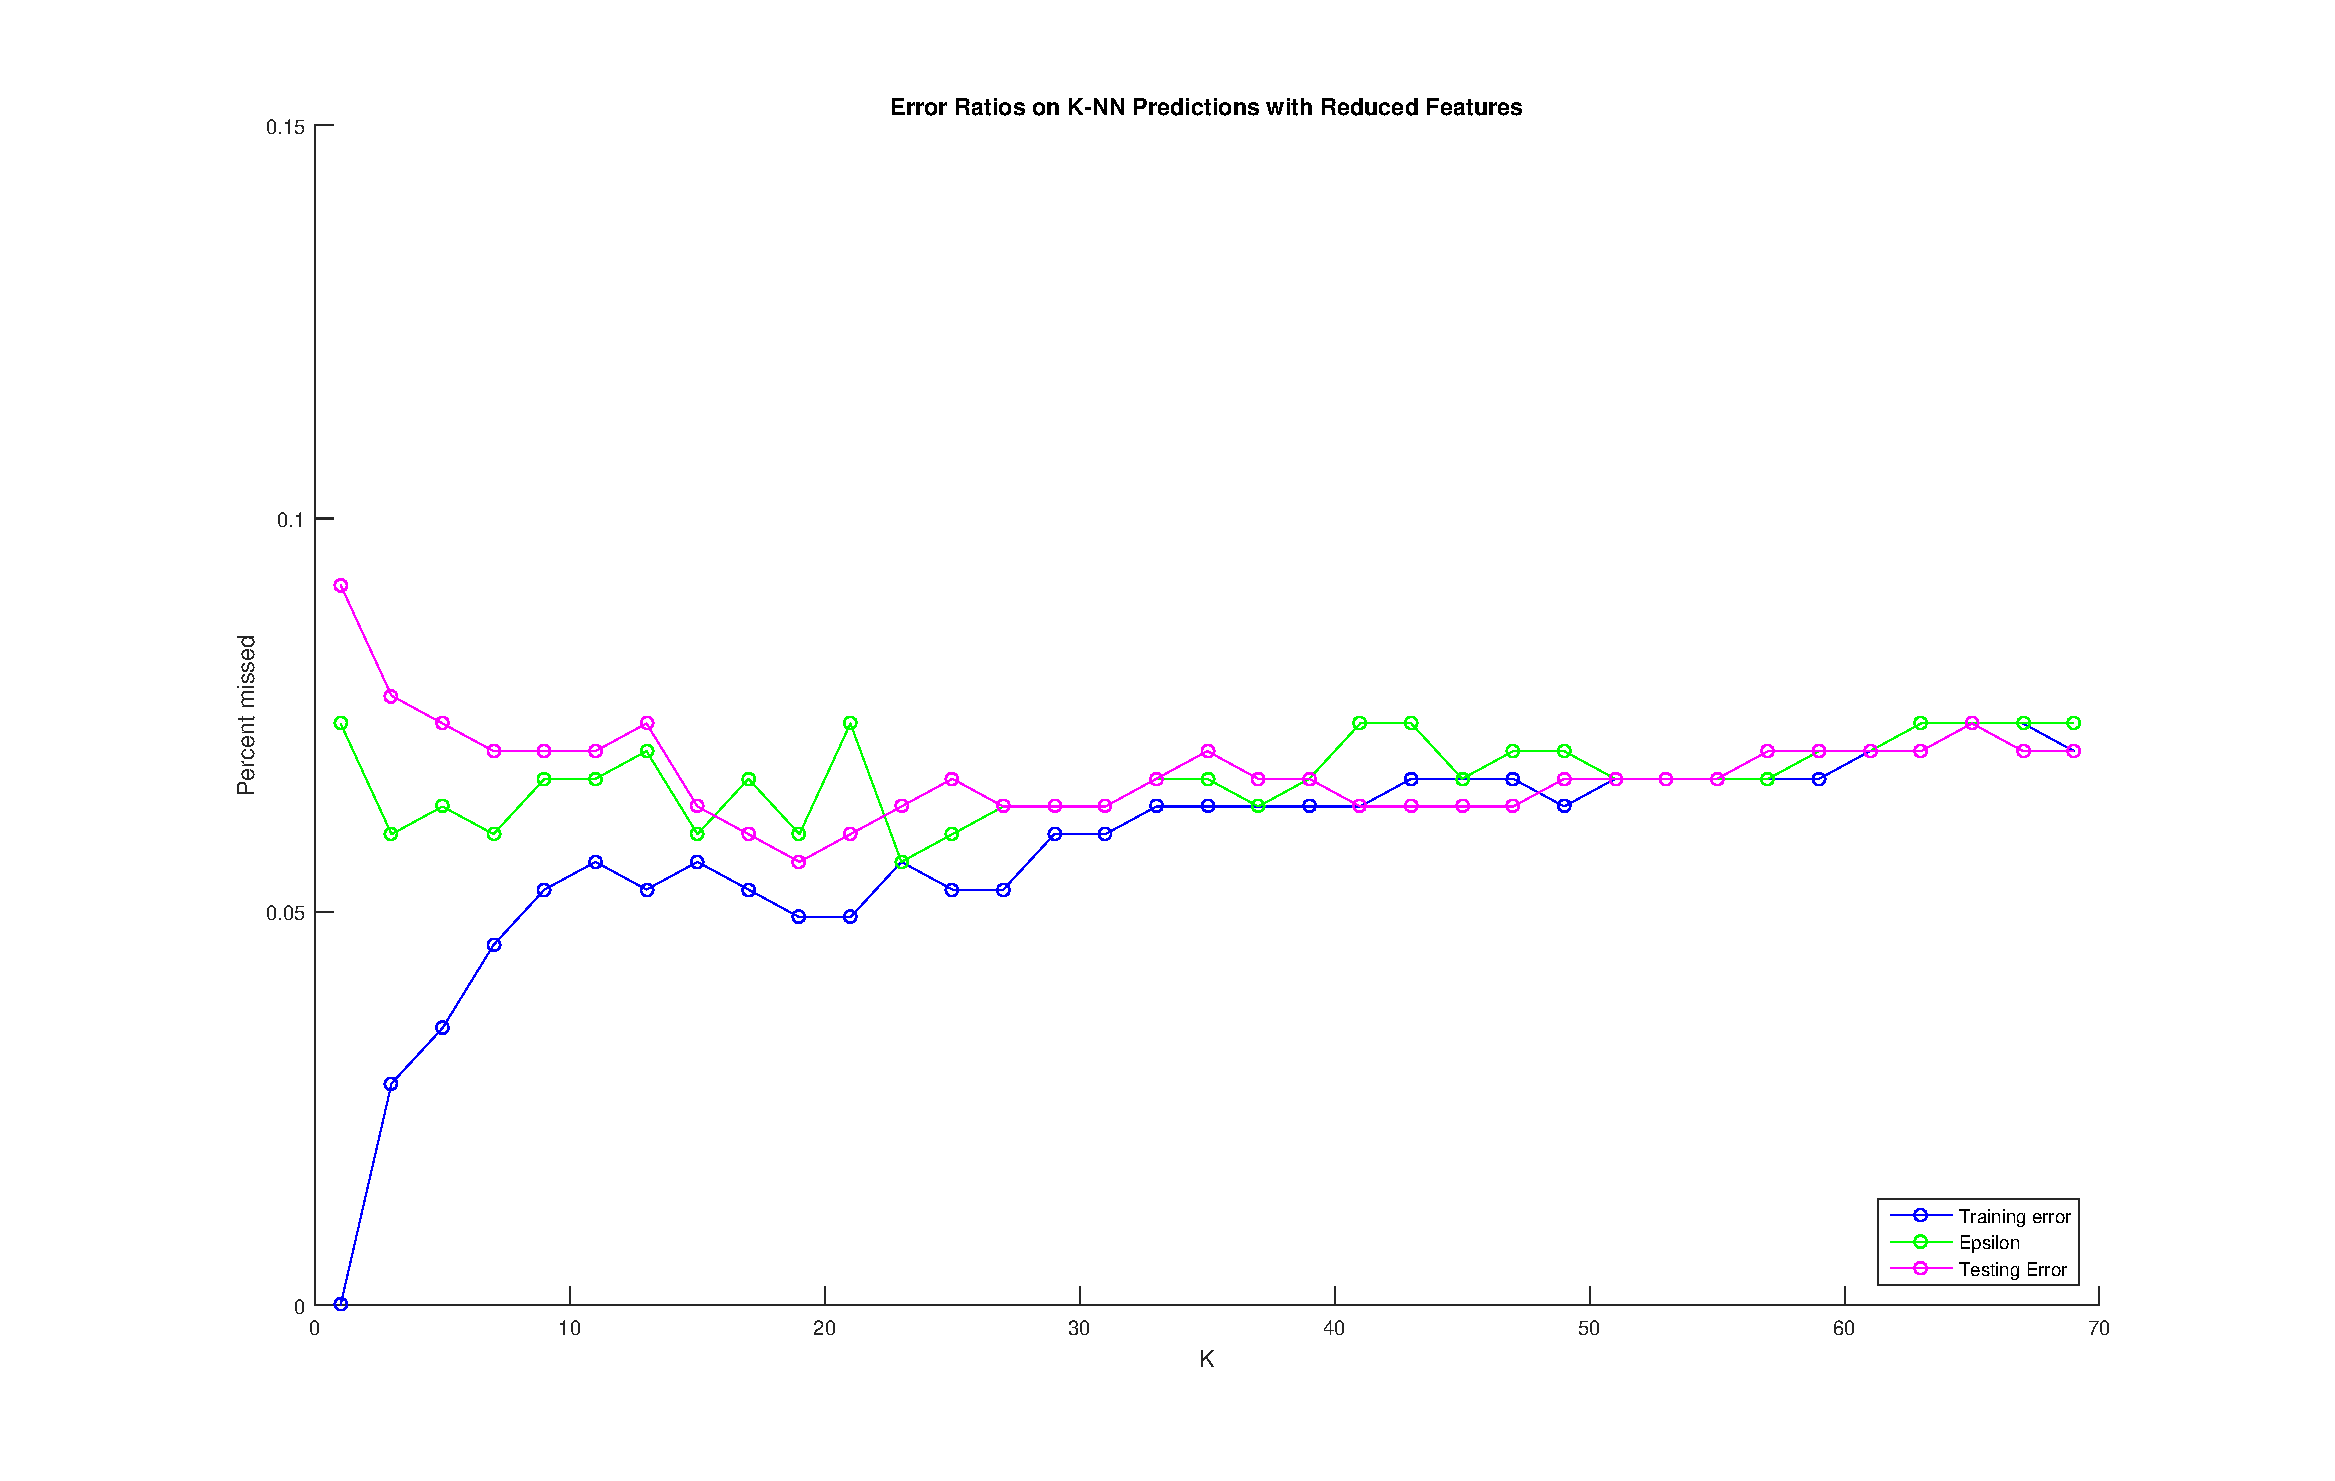
\includegraphics[scale=0.4]{reduced.eps} 
		\end{center}  
		\label{fig:M3}
	\end{figure}

As we can see this didn't end up improving performance but it doesn't really hurt it much either. Since the new model only needs to gather 6 features to make this prediction, depending on the costs or difficulty of gathering the other feature data this might be a much better option for future model generation and prediction.

\newpage


	
	%\bibliography{myCitations} 
	%\bibliographystyle{abbrv}
	
\end{document} 